% Artigo XXI ERIAC - CE A2. Compile no Overleaf (pdfLaTeX + BibTeX) ou com latexmk -pdf.
% Os números vêm de numeros.tex e as tabelas de tabelas/, ambos gerados por gerar_artigo.py.
\documentclass[11pt,a4paper]{article}
\usepackage[utf8]{inputenc}
\usepackage[T1]{fontenc}
\usepackage[brazil]{babel}
\usepackage{lmodern}
\usepackage{textcomp}
\usepackage{icomma}
\usepackage[a4paper,top=2.5cm,bottom=2.5cm,left=2.5cm,right=2.5cm]{geometry}
\usepackage{graphicx}
\usepackage{booktabs}
\usepackage{amsmath,amssymb}
\usepackage{xcolor}
\usepackage[labelsep=period,font=small]{caption}
\usepackage{tikz}
\usetikzlibrary{arrows.meta,positioning}
\usepackage[hidelinks]{hyperref}
\usepackage{titlesec}

\graphicspath{{figuras/}}
% Gerado por gerar_artigo.py a partir de saida/. Não edite à mão.
\newcommand{\NImagens}{255}
\newcommand{\NCores}{253}
\newcommand{\MaxIdxSaudavel}{0,136}
\newcommand{\MaxIdxSCoitenta}{0,088}
\newcommand{\SatSCseiscentos}{0,03\%}
\newcommand{\VizMesmaClasse}{98,8\%}
\newcommand{\VizAdjacente}{35,7\%}
\newcommand{\FUmOriginal}{0,997}
\newcommand{\MAEOriginal}{6,16}
\newcommand{\FUmBlocosHib}{0,982}
\newcommand{\MAEBlocosHib}{6,9}
\newcommand{\FUmBlocosTriv}{0,974}
\newcommand{\MAEBlocosTriv}{9,8}
\newcommand{\FUmBlocosPos}{0,50}
\newcommand{\MAEBlocosDino}{10,8}
\newcommand{\MAEBlocosInd}{5,3}
\newcommand{\CobBlocosHib}{0,929}
\newcommand{\MeiaBlocosHib}{17}
\newcommand{\OODBlocosHib}{2,3\%}
\newcommand{\InterpHib}{14,8}
\newcommand{\InterpHibPior}{25,8}
\newcommand{\InterpInd}{38,8}
\newcommand{\InterpIndPior}{80,0}
\newcommand{\InterpDino}{21,4}
\newcommand{\InterpDinoPior}{34,5}
\newcommand{\InterpTriv}{34,7}
\newcommand{\InterpTrivPior}{60,8}
\newcommand{\InterpMB}{17,0}
\newcommand{\InterpMBPior}{22,9}
\newcommand{\InterpMob}{18,0}
\newcommand{\InterpMobPior}{27,7}
\newcommand{\InterpHibVum}{19,5}
\newcommand{\InterpHibVumPior}{39,7}
\newcommand{\InterpHibPiorCond}{SC80}
\newcommand{\InterpHibNivel}{97\%}
\newcommand{\InterpHibCob}{91\%}
\newcommand{\InterpHibMeia}{37}
\newcommand{\InterpHibSCtrezentosvinte}{6,0}
\newcommand{\CampTriv}{91,0}
\newcommand{\CampTrivOOD}{33\%}
\newcommand{\CampDino}{39,6}
\newcommand{\CampDinoOOD}{62\%}
\newcommand{\CampHib}{33,6}
\newcommand{\CampHibOOD}{67\%}
\newcommand{\CampMB}{31,3}
\newcommand{\CampMBOOD}{100\%}
\newcommand{\CampAAlfa}{0,27}
\newcommand{\AninhadaMAE}{18,5}
\newcommand{\AninhadaEscolhas}{5}
\newcommand{\ZooN}{44}
\newcommand{\ZooMelhor}{13,6}
\newcommand{\ZooKernelMin}{41}
\newcommand{\PHibDino}{0,016}
\newcommand{\NHibDino}{7}
\newcommand{\PHibInd}{0,031}
\newcommand{\NHibInd}{6}
\newcommand{\PMBHib}{0,69}
\newcommand{\ICHibInf}{9,6}
\newcommand{\ICHibSup}{20,5}
\newcommand{\RobIndSemFiltroRuidoFUm}{0,38}
\newcommand{\RobIndRuidoFUm}{0,66}
\newcommand{\RobIndSemFiltroTransl}{18,7}
\newcommand{\RobIndTransl}{6,3}
\newcommand{\AumMBSevAntes}{18,0}
\newcommand{\AumMBSevDepois}{13,9}
\newcommand{\AumMBCampAntes}{33,0}
\newcommand{\AumMBCampDepois}{19,4}
\newcommand{\AumMBRuidoAntes}{36,7}
\newcommand{\AumMBRuidoDepois}{16,5}
\newcommand{\AumHibSevDepois}{19,2}
\newcommand{\DerivaMax}{18}
\newcommand{\DerivaRhoMax}{0,91}
\newcommand{\SensMAEMin}{6,1}
\newcommand{\SensMAEMax}{9,0}
\newcommand{\SensFUmMin}{0,969}
\newcommand{\OclMobMin}{78\%}
\newcommand{\OclMobMax}{85\%}
\newcommand{\OclIndMin}{47\%}
\newcommand{\OclIndMax}{100\%}
\newcommand{\MotorFUm}{0,997}
\newcommand{\MotorFUmTriv}{0,942}
\newcommand{\MotorFUmPos}{0,54}
\newcommand{\MotorMAE}{0,85}
\newcommand{\MotorSevMob}{4,1}
\newcommand{\MotorSevPos}{3,8}
\newcommand{\MotorCores}{242}
\newcommand{\VerifMin}{99,2\%}
\newcommand{\VerifMax}{100\%}
\newcommand{\RelAprovados}{255}
\newcommand{\AppMeia}{22}


% Estilo do rascunho: seções numeradas em caixa alta, tabelas em algarismos romanos.
\titleformat{\section}{\normalfont\bfseries}{\thesection}{0.6em}{\MakeUppercase}
\titleformat{\subsection}{\normalfont\bfseries}{\thesubsection}{0.6em}{}
\renewcommand{\thetable}{\Roman{table}}
\captionsetup[table]{name=TABELA,labelfont=bf,justification=centering}
\captionsetup[figure]{name=Fig.,labelfont=bf}
\newcommand{\todo}[1]{\textcolor{red}{[TODO: #1]}}
\setlength{\parskip}{0.35em}

\begin{document}

\begin{center}
{\small\bfseries XXI ERIAC\\ VIGÉSIMO PRIMEIRO ENCONTRO REGIONAL IBERO-AMERICANO DO CIGRE}\\[2pt]
{\small 23 a 27 de maio de 2027 \hfill Ciudad del Este, Paraguay \hfill A2}\\[2pt]
{\small Comitê de Estudos A2 -- Transformadores}\\[14pt]
{\large\bfseries Diagnóstico da Severidade de Curtos entre Espiras em Transformadores: Uma Solução Baseada em Termografia, Visão Computacional e LLMs}\\[10pt]
\todo{autor principal}$^{*}$ \quad \todo{coautores}\\
{\small \todo{entidade: UFCG} \quad $^{*}$\todo{e-mail}}
\end{center}

\noindent\textbf{Resumo} -- Este trabalho avalia o diagnóstico de curtos entre espiras e a estimativa da sua severidade em um transformador monofásico de bancada a partir de \NImagens{} termogramas RGB não radiométricos, com a condição saudável e oito níveis de curto. A paleta de cores da câmera (\NCores{} cores) foi recuperada sem rótulos, o que permite converter cada pixel em um índice ordinal, sem atribuir temperatura. Representações DINOv2 congeladas foram combinadas a indicadores relativos calculados sobre esse índice. O protocolo de avaliação inclui blocos temporais com purga, retirada integral de uma severidade, retirada integral de uma campanha de aquisição, linha de base trivial e controle de enquadramento. Dentro das sessões de gravação, até uma miniatura de 16$\times$12 pixels atinge F1-macro de \FUmBlocosTriv{}, o que torna esse teste pouco discriminante. Com a severidade ausente do treinamento, o método híbrido errou em média \InterpHib{} espiras de 600 (pior caso \InterpHibPior{}) e acertou o nível nominal em \InterpHibNivel{} das imagens, com ganho significativo sobre o DINOv2 isolado (\NHibDino{} de 7 níveis, \textit{p}~=~\PHibDino) e sobre os indicadores isolados. Um intervalo conformal acompanha cada estimativa, e um detector de domínio sinaliza imagens diferentes das de treinamento. Um LLM redige o relatório a partir do diagnóstico estruturado; as recomendações vêm de regras, e um verificador automático detectou de \VerifMin{} a \VerifMax{} dos erros injetados nos relatórios. O mesmo pipeline, sem ajustes, classificou 11 condições de um motor de indução com F1-macro de \MotorFUm{}.

\noindent\textbf{Palavras-chave} -- Transformador; Curto entre espiras; Termografia infravermelha; Visão computacional; Incerteza conformal; Modelos de linguagem; Diagnóstico de falhas.

\section{Introdução}

Curtos entre espiras alteram a distribuição de perdas no enrolamento e, com ela, o padrão de aquecimento do equipamento. A termografia infravermelha é uma técnica de inspeção não invasiva consolidada na manutenção de equipamentos elétricos \cite{bagavathiappan2013}. Grande parte dos termogramas disponíveis, porém, é exportada como imagem colorida, sem a matriz radiométrica: a cor indica a posição na escala da câmera, mas não a temperatura. \todo{acrescentar 2 ou 3 referências de termografia e de detecção de curto entre espiras em transformadores}

Um estudo preliminar deste grupo, com o dataset público de Najafi \textit{et al.} \cite{najafi2020trafo}, obteve F1-macro de \FUmOriginal{} e erro médio de \MAEOriginal{} espiras na estimativa da severidade. Esses números foram reproduzidos exatamente neste trabalho, mas vinham de uma validação cruzada por imagem, na qual quadros consecutivos e quase idênticos de uma mesma gravação caem no treino e no teste. Em dados com estrutura temporal, esse tipo de divisão superestima o desempenho \cite{roberts2017cv}.

A pergunta deste trabalho é: em que medida é possível estimar a severidade de um curto entre espiras, inclusive para uma severidade ou uma sessão de gravação ausentes do treinamento, a partir de termogramas não radiométricos? As contribuições são:
(i) a recuperação da paleta da câmera sem rótulos e o uso do índice ordinal resultante como base de indicadores relativos;
(ii) um protocolo de avaliação que separa o que o modelo aprende do padrão térmico do que ele memoriza da sessão de gravação;
(iii) a evidência de que a combinação de DINOv2 com indicadores generaliza melhor que cada componente;
(iv) intervalos conformais e detecção de imagens fora do domínio;
(v) uma camada de relatório por LLM restrita e verificada automaticamente; e
(vi) uma ferramenta de aplicação e o teste do mesmo pipeline em um segundo equipamento.

\section{Dados e suas limitações}

O subconjunto do transformador contém \NImagens{} imagens BMP de 320$\times$240 pixels: 22 da condição saudável e 26 a 40 de cada condição com 80, 160, 240, 320, 400, 480, 560 e 600 espiras em curto, de um total de 600 \cite{najafi2020trafo}. O equipamento é descrito como transformador monofásico de 1\,kW e 220\,V, e as imagens foram adquiridas em bancada com uma câmera Dali-tech T8. O dataset não informa o enrolamento associado às 600 espiras, a corrente no laço em curto, a carga nem o tempo de aquecimento.

\textbf{Paleta.} As imagens usam exatamente \NCores{} cores, todas sobre uma única curva no espaço RGB (paleta do tipo \textit{ironbow}). A ordem das cores foi recuperada pelo caminho mais longo da árvore geradora mínima das cores, orientado do escuro para o claro. Cada pixel recebe assim um índice ordinal entre 0 e 1. Como a faixa de temperatura configurada na câmera não é conhecida, o índice não é convertido em graus, e nenhuma diferença de índice é tratada como diferença de temperatura.

\textbf{Campanhas de aquisição.} A numeração dos arquivos continua de uma pasta para a seguinte quando as condições foram gravadas em sequência. Isso revela quatro campanhas: A (saudável), B (80 e 160 espiras), C (240 e 320) e D (400 a 600). O enquadramento e o fundo mudam entre campanhas (Fig.~\ref{fig:indicadores}). A condição saudável existe em uma única campanha, e seu índice máximo médio (\MaxIdxSaudavel) é maior que o da condição com 80 espiras (\MaxIdxSCoitenta), um efeito de campanha e não do defeito. Consequentemente, a detecção da condição saudável não pode ser separada da identificação da campanha A.

\textbf{Dependência entre quadros.} Para \VizMesmaClasse{} das imagens, a imagem mais parecida (similaridade de cosseno entre embeddings DINOv2) é da mesma classe, e em \VizAdjacente{} dos casos é o quadro imediatamente adjacente. A saturação no fim da paleta é desprezível (\SatSCseiscentos{} da região do transformador no SC600).

\begin{figure}[t]
\centering
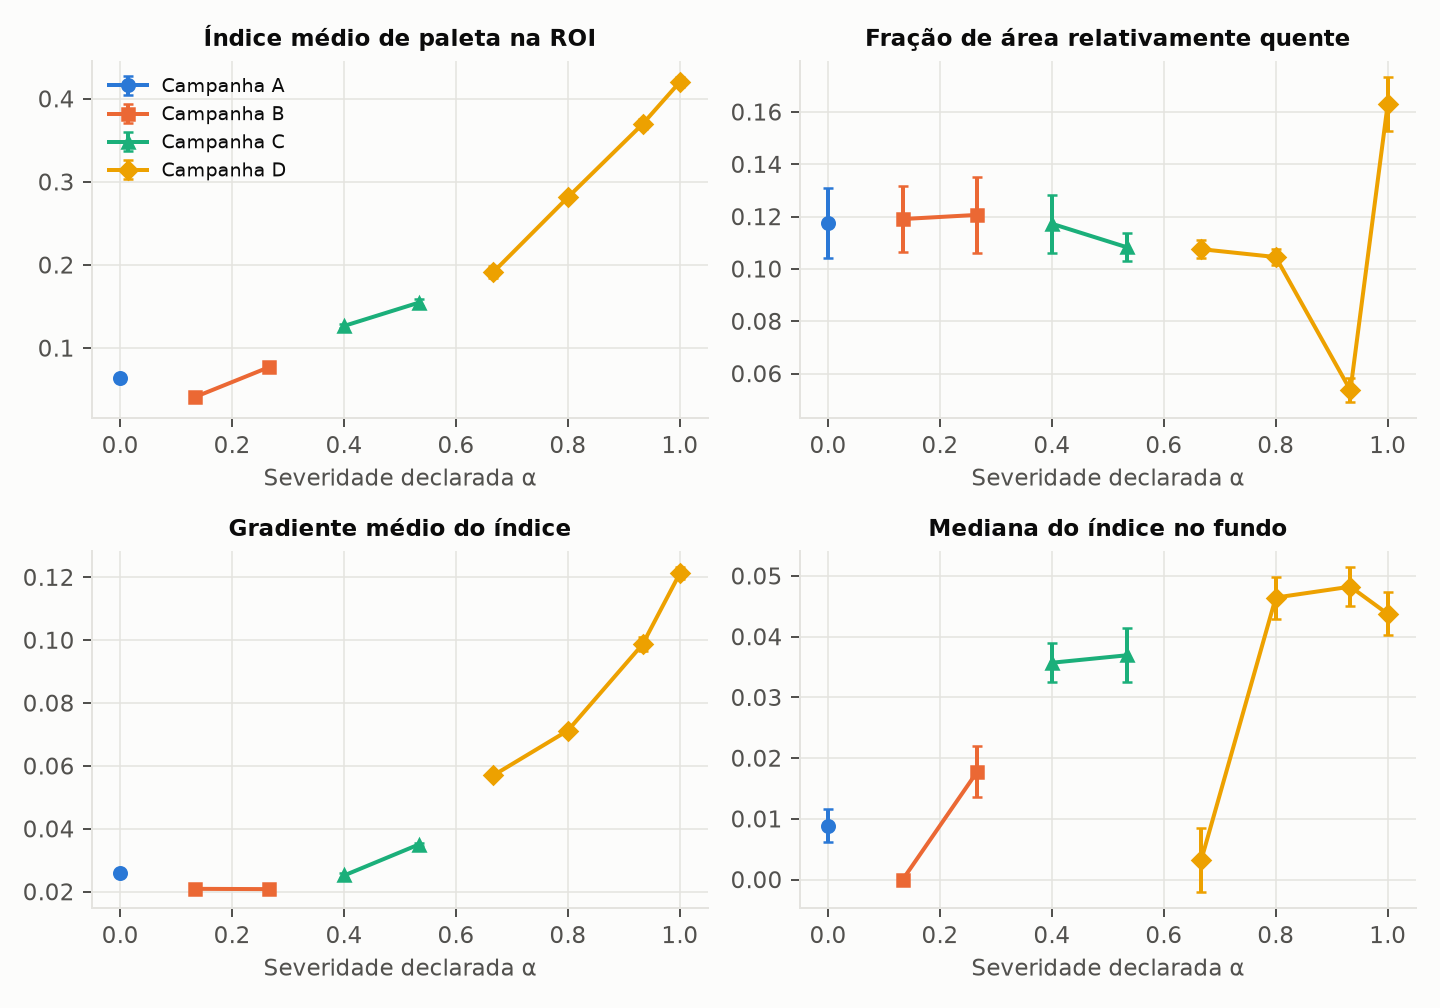
\includegraphics[width=0.82\linewidth]{fig_indicadores_severidade.png}
\caption{Indicadores relativos por severidade declarada, coloridos por campanha de aquisição. Os saltos entre campanhas, sobretudo no índice do fundo, mostram o fator de confusão entre sessão de gravação e severidade.}
\label{fig:indicadores}
\end{figure}

\section{Metodologia}

\subsection{Severidade}
A severidade contínua é $\alpha = N_f/N_{\mathrm{total}}$, com $N_{\mathrm{total}}=600$. A tarefa binária separa a condição saudável das demais; a multiclasse usa as nove condições; a regressão estima $\alpha\in[0,1]$, e o número de espiras é $\hat{N}_f = 600\,\hat{\alpha}$.

\subsection{Indicadores de paleta}
A região do transformador é segmentada pela distância CIELAB à cor mediana dos quatro cantos da imagem, seguida de operações morfológicas e da maior componente conectada. Sobre o índice de paleta, filtrado por uma mediana 5$\times$5 para absorver ruído de sensor, são calculados 39 indicadores: estatísticas do índice na região (média, percentis, desvio, assimetria), fração de área relativamente aquecida (índice $\geq 0{,}65$), fração saturada, contraste com o fundo, posição e dispersão do ponto quente aparente, gradiente, entropia e um histograma de 16 faixas.

\subsection{Representações e modelos}
Foram usados dois extratores pré-treinados e congelados: DINOv2 ViT-S/14 \cite{oquab2023dinov2} (384 dimensões) e MobileNetV3-small \cite{howard2019mobilenetv3} (576 dimensões), com entrada RGB 224$\times$224 e normalização ImageNet. A classificação usa regressão logística com pesos balanceados, e a regressão de $\alpha$ usa Ridge \cite{hoerl1970ridge}, ambas com padronização \cite{pedregosa2011sklearn}. Os hiperparâmetros são escolhidos por validação interna dentro de cada dobra de treino \cite{varma2006bias,cawley2010}.

\subsection{Protocolo de avaliação}
Quatro esquemas de divisão foram usados:
\textit{(a) aleatória por imagem}, apenas para medir o vazamento entre quadros vizinhos;
\textit{(b) blocos temporais}: cada condição é dividida em cinco trechos contíguos, cada dobra testa um trecho de todas as condições, e o quadro vizinho à fronteira é retirado do treino (purga);
\textit{(c) severidade não vista}: cada uma das sete severidades intermediárias sai inteira do treino, e a validação interna também é agrupada por nível;
\textit{(d) campanha não vista}: uma campanha inteira sai do treino, junto com seu enquadramento.
Todos os métodos foram comparados com uma linha de base (a imagem em cinza reduzida a 16$\times$12 pixels) e um controle que contém apenas a posição e o tamanho da região segmentada. Diferenças entre métodos na severidade não vista foram testadas com o teste de Wilcoxon pareado sobre os sete níveis \cite{wilcoxon1945}, cujo menor valor-p bilateral possível é 0,016.

Para medir o efeito de escolher um modelo entre muitos, 44 combinações de features e regressores (Ridge, PLS \cite{wold2001pls}, PCA seguida de Ridge, Kernel Ridge, SVR, processo gaussiano e médias de modelos) foram avaliadas também em uma seleção aninhada: para cada severidade retirada, o modelo é escolhido pelo erro de interpolação dentro do treino, e só então a severidade retirada é prevista.

\subsection{Incerteza e domínio}
Cada estimativa de $\alpha$ recebe um intervalo conformal de 90\% \cite{vovk2005,lei2018conformal,angelopoulos2021}, calibrado com resíduos fora da dobra dentro do treino. Na severidade não vista, os resíduos vêm da retirada, um de cada vez, dos níveis interiores do treino. Um detector de domínio mede a distância média aos cinco vizinhos mais próximos no conjunto de treino \cite{sun2022knn}; acima do percentil 99 das distâncias do próprio treino, a imagem é considerada fora do domínio.

\subsection{Camada de relatório}
O LLM recebe um registro estruturado com a condição estimada, $\hat\alpha$ e seu intervalo, a confiança, o controle de qualidade (domínio, coerência visual, concordância entre módulos), indicadores relativos e limitações; o rótulo verdadeiro não é incluído. A recomendação é escolhida por regras determinísticas a partir de $\hat\alpha$; fora do domínio, ou com módulos discordantes, a regra encaminha a imagem a um especialista. As faixas de recomendação são ilustrativas e não normativas; as ações sugerem ensaios elétricos confirmatórios, como relação de transformação e corrente de excitação \cite{ieeec57152}. O LLM apenas redige o texto (Fig.~\ref{fig:relatorio}). Um verificador confere o texto contra o registro: todo número citado deve existir no registro, nenhuma unidade de temperatura pode aparecer ao lado de um número, a recomendação deve ser a da regra e as limitações devem estar presentes. Isso limita as alucinações típicas de modelos de linguagem \cite{ji2023hallucination}.

\begin{figure}[t]
\centering
\begin{tikzpicture}[node distance=4mm, caixa/.style={draw, rounded corners=2pt, align=center, font=\footnotesize, minimum height=10mm, text width=22mm}, >={Stealth[length=2mm]}]
\node[caixa] (img) {Termograma\\RGB};
\node[caixa, right=of img] (mod) {Modelos\\$\hat\alpha$, intervalo,\\domínio};
\node[caixa, right=of mod] (reg) {Registro\\estruturado};
\node[caixa, right=of reg] (reg2) {Regra de\\recomendação};
\node[caixa, right=of reg2, draw=violet, thick] (llm) {LLM\\(só redige)};
\node[caixa, below=6mm of llm] (ver) {Verificador\\automático};
\node[caixa, left=of ver] (sai) {Relatório\\aprovado ou\\reprovado};
\draw[->] (img) -- (mod); \draw[->] (mod) -- (reg); \draw[->] (reg) -- (reg2); \draw[->] (reg2) -- (llm);
\draw[->] (llm) -- (ver); \draw[->] (ver) -- (sai); \draw[->, dashed] (reg) |- (ver);
\end{tikzpicture}
\caption{Camada de relatório. Números e recomendação são produzidos antes do LLM; o verificador compara o texto com o registro.}
\label{fig:relatorio}
\end{figure}

\section{Resultados e discussão}

\subsection{Validação dentro das sessões de gravação}
A Tabela~\ref{tab:validacao} mostra que a divisão por blocos temporais quase não altera os números em relação à divisão aleatória. Isso não indica que o problema seja resolvido: a linha de base de 16$\times$12 pixels atinge F1-macro de \FUmBlocosTriv{} e erro de \MAEBlocosTriv{} espiras, e o DINOv2 isolado (\MAEBlocosDino{} espiras) fica pior que ela. O controle de posição, sem nenhum padrão térmico, atinge F1-macro de \FUmBlocosPos{}, contra 0,11 do acaso. Dentro de uma sessão, o problema está no teto e não discrimina métodos. O intervalo conformal do híbrido cobriu \CobBlocosHib{} dos casos, com meia-largura média de \MeiaBlocosHib{} espiras.

\begin{table}[t]
\centering
\caption{Validação cruzada aninhada: divisão aleatória por imagem e por blocos temporais (F1-macro das 9 condições; MAE da severidade em espiras de 600)}
\label{tab:validacao}
\small\begin{tabular}{lrrrr}
\toprule
Features & F1 aleat. & F1 blocos & MAE aleat. & MAE blocos \\
\midrule
Miniatura 16$\times$12 (linha de base) & 0,991 & 0,974 & 7,7 & 9,8 \\
Posição do objeto (controle) & 0,605 & 0,499 & 91,2 & 90,9 \\
Indicadores v1 (rascunho) & 0,995 & 0,995 & 4,7 & 5,5 \\
Indicadores de paleta & 1,000 & 1,000 & 4,0 & 5,3 \\
MobileNetV3 & 1,000 & 0,980 & 6,3 & 8,1 \\
DINOv2 & 0,987 & 0,982 & 9,0 & 10,8 \\
DINOv2 + indicadores v1 & 0,996 & 0,996 & 6,3 & 7,2 \\
\textbf{DINOv2 + indicadores de paleta} & \textbf{0,996} & \textbf{0,982} & \textbf{5,7} & \textbf{6,9} \\
MobileNetV3 + indicadores de paleta & 1,000 & 0,980 & 5,2 & 6,9 \\
\bottomrule
\end{tabular}

\end{table}

\subsection{Severidade não vista no treinamento}
Com uma severidade intermediária inteira fora do treino (Tabela~\ref{tab:interpolacao} e Fig.~\ref{fig:interp}), o híbrido DINOv2 + indicadores de paleta errou em média \InterpHib{} espiras (IC 95\% por reamostragem dos níveis: \ICHibInf{} a \ICHibSup), com pior caso de \InterpHibPior{} espiras (\InterpHibPiorCond), e acertou o nível nominal mais próximo em \InterpHibNivel{} das imagens. O ganho sobre o DINOv2 isolado ocorreu nos \NHibDino{} níveis (\textit{p}~=~\PHibDino), e sobre os indicadores isolados em \NHibInd{} de 7 (\textit{p}~=~\PHibInd). Os indicadores isolados falham nas pontas da interpolação, e a linha de base, que ia bem dentro das sessões, erra \InterpTriv{} espiras. A combinação com a MobileNetV3, que roda inteiramente no computador do usuário, não diferiu significativamente do híbrido com DINOv2 (\textit{p}~=~\PMBHib; com sete níveis, o teste tem pouco poder para afirmar equivalência). O caso do SC320, destacado no estudo preliminar, ficou em \InterpHibSCtrezentosvinte{} espiras, abaixo da média, e não deve ser tomado como típico. O intervalo conformal calibrado com níveis retirados cobriu \InterpHibCob{} dos casos, com meia-largura média de \InterpHibMeia{} espiras.

\begin{table}[t]
\centering
\caption{Severidade não vista: erro médio e pior caso (espiras), acerto do nível nominal e cobertura do intervalo de 90\%}
\label{tab:interpolacao}
\small\begin{tabular}{lrrrr}
\toprule
Features & MAE médio & Pior caso & Nível certo & Cobertura IC 90\% \\
\midrule
Miniatura 16$\times$12 (linha de base) & 34,7 & 60,8 (SC240) & 49\% & 89\% \\
Posição do objeto (controle) & 114,0 & 243,5 (SC560) & 20\% & 86\% \\
Indicadores v1 (rascunho) & 33,0 & 80,0 (SC80) & 58\% & 86\% \\
Indicadores de paleta & 38,8 & 80,0 (SC80) & 56\% & 86\% \\
MobileNetV3 & 18,0 & 27,7 (SC320) & 92\% & 91\% \\
DINOv2 & 21,4 & 34,5 (SC240) & 85\% & 84\% \\
DINOv2 + indicadores v1 & 19,5 & 39,7 (SC80) & 91\% & 83\% \\
\textbf{DINOv2 + indicadores de paleta} & \textbf{14,8} & \textbf{25,8 (SC80)} & \textbf{97\%} & \textbf{91\%} \\
MobileNetV3 + indicadores de paleta & 17,0 & 22,9 (SC320) & 98\% & 93\% \\
\bottomrule
\end{tabular}

\end{table}

\begin{figure}[t]
\centering
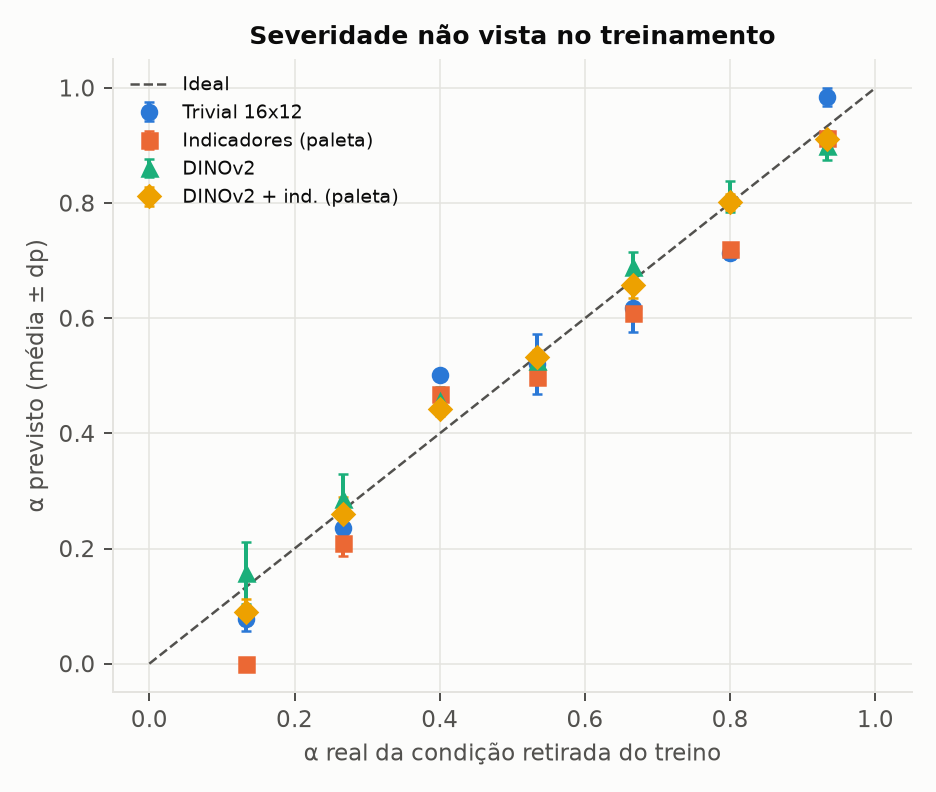
\includegraphics[width=0.48\linewidth]{fig_interpolacao.png}\hfill
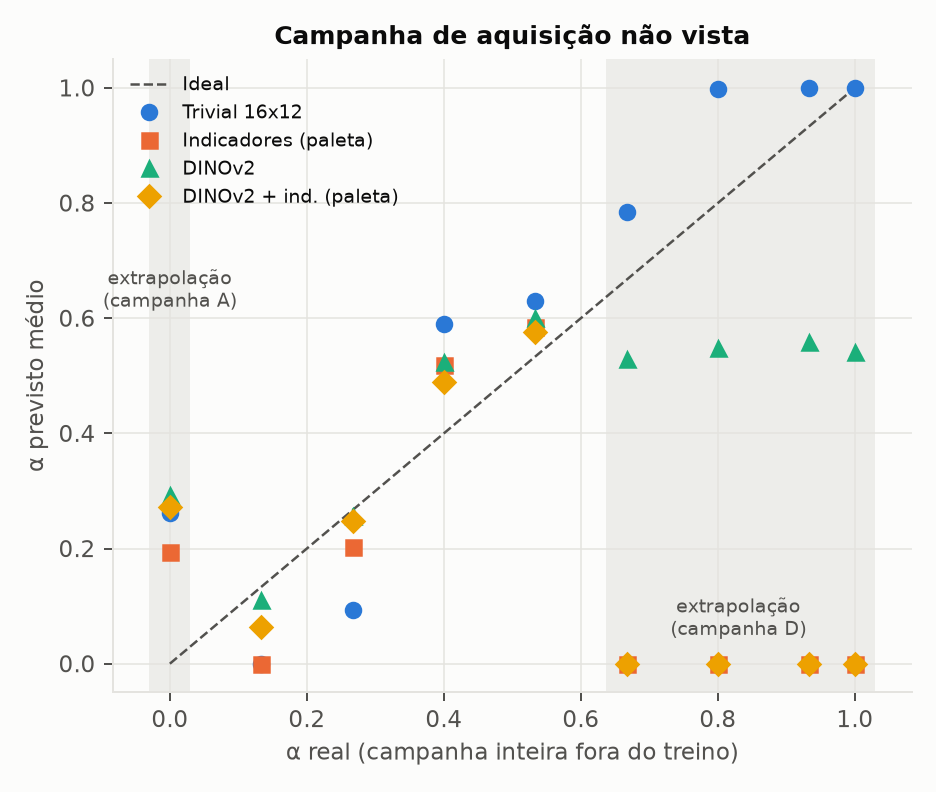
\includegraphics[width=0.48\linewidth]{fig_campanhas.png}
\caption{Esquerda: $\alpha$ previsto para cada severidade retirada do treino. Direita: $\alpha$ previsto com uma campanha de aquisição inteira fora do treino; as faixas cinza indicam extrapolação.}
\label{fig:interp}
\end{figure}

\textbf{Busca de modelos.} Entre as \ZooN{} combinações avaliadas, a melhor obteve \ZooMelhor{} espiras quando escolhida olhando o próprio teste (Tabela~\ref{tab:zoo}). Os regressores com núcleo (Kernel Ridge, SVR) extrapolaram mal, com erros acima de \ZooKernelMin{} espiras. Na seleção aninhada, que escolhe sem ver a severidade retirada, o modelo escolhido variou entre \AninhadaEscolhas{} combinações ao longo dos níveis, e o erro resultante foi de \AninhadaMAE{} espiras, maior que o do híbrido definido de antemão. Com sete níveis de severidade, buscar o melhor modelo não melhorou o resultado de forma confiável.

\begin{table}[t]
\centering
\caption{As seis melhores combinações na severidade não vista (escolhidas olhando o teste, portanto otimistas) e seu erro com campanha não vista}
\label{tab:zoo}
\small\begin{tabular}{llrrr}
\toprule
Features & Regressor & Sev. nova & Pior & Camp. nova \\
\midrule
DINOv2 + indicadores sem cena & Ridge & 13,6 & 26,5 & 32,9 \\
Média de modelos & média DINOv2 e MobileNet & 14,7 & 25,8 & 19,5 \\
DINOv2 + indicadores de paleta & Ridge & 14,8 & 25,8 & 33,6 \\
DINOv2 + indicadores sem cena & PLS & 16,6 & 42,5 & 30,9 \\
MobileNetV3 + indicadores de paleta & Ridge & 17,0 & 22,9 & 31,3 \\
DINOv2 + indicadores de paleta & PLS & 17,2 & 46,2 & 44,6 \\
\bottomrule
\end{tabular}

\end{table}

\subsection{Campanha de aquisição não vista}
Retirar uma campanha inteira retira também o seu enquadramento (Tabela~\ref{tab:campanha}). A linha de base desaba para \CampTriv{} espiras, pois dependia da sessão. O híbrido errou \CampHib{} espiras nas campanhas intermediárias (B e C), e a extrapolação falhou: sem a campanha A, a condição saudável foi prevista com $\alpha\approx{}$\,\CampAAlfa, e sem a campanha D as previsões saturaram em $\alpha=1$. O detector de domínio marcou \CampHibOOD{} dessas imagens, o que faz a camada de relatório substituir a recomendação pelo encaminhamento a um especialista. Considerando as quatro campanhas, inclusive as de extrapolação, o detector rejeitou \AbstCampFracRejeitada{} das imagens; as rejeitadas tiveram erro médio de \AbstCampRejeitadas{} espiras, contra \AbstCampAceitas{} das aceitas (correlação de Spearman de \AbstCampRho{} entre o escore de domínio e o erro). Com severidade nova em campanha conhecida, a separação foi fraca (\AbstSevAceitas{} contra \AbstSevRejeitadas{} espiras): o detector responde sobretudo a mudanças de cena, e é nesses casos que ele evita os erros mais graves.

\begin{table}[t]
\centering
\caption{Campanha não vista (erro em espiras) e fração das imagens marcadas como fora do domínio}
\label{tab:campanha}
\small\begin{tabular}{lrrrr}
\toprule
Features & Camp. B & Camp. C & B + C & Fora do domínio \\
\midrule
Miniatura 16$\times$12 (linha de base) & 92,1 & 88,7 & 91,0 & 33\% \\
Posição do objeto (controle) & 142,3 & 131,7 & 135,9 & 4\% \\
Indicadores de paleta & 59,3 & 51,2 & 54,5 & 99\% \\
MobileNetV3 & 46,5 & 18,9 & 33,0 & 100\% \\
DINOv2 & 23,5 & 57,2 & 39,6 & 62\% \\
\textbf{DINOv2 + indicadores de paleta} & \textbf{29,2} & \textbf{39,6} & \textbf{33,6} & \textbf{67\%} \\
MobileNetV3 + indicadores de paleta & 46,2 & 16,0 & 31,3 & 100\% \\
\bottomrule
\end{tabular}

\end{table}

\subsection{Robustez, aumento de dados e deriva temporal}
O filtro de mediana no índice de paleta elevou o F1-macro dos indicadores sob ruído gaussiano de \RobIndSemFiltroRuidoFUm{} para \RobIndRuidoFUm{}, e reduziu o erro sob translação de \RobIndSemFiltroTransl{} para \RobIndTransl{} espiras, sem piorar as imagens limpas. Treinar com cópias perturbadas das imagens (intensidade menor que a do teste e outra semente) tornou a MobileNetV3 robusta: sob ruído, o erro caiu de \AumMBRuidoAntes{} para \AumMBRuidoDepois{} espiras (Tabela~\ref{tab:aumento}). De forma exploratória, o aumento de dados também reduziu o erro da MobileNetV3 na severidade não vista (\AumMBSevAntes{} para \AumMBSevDepois{}) e na campanha não vista (\AumMBCampAntes{} para \AumMBCampDepois{}), possivelmente por reduzir a dependência do enquadramento. Para a combinação com indicadores, o mesmo não ocorreu (\AumHibSevDepois{} espiras na severidade não vista).

\begin{table}[t]
\centering
\caption{Efeito do aumento de dados: erro (espiras) em imagens limpas e perturbadas (blocos temporais) e na severidade e na campanha não vistas}
\label{tab:aumento}
\footnotesize\begin{tabular}{lrrrrrrr}
\toprule
Modelo & Limpa & Ruído & Desfoque & Transl. & Rotação & Sev. nova & Camp. nova \\
\midrule
MobileNetV3, sem aumento & 8,1 & 36,7 & 24,8 & 14,5 & 12,5 & 18,0 & 33,0 \\
\textbf{MobileNetV3, com aumento} & \textbf{6,8} & \textbf{16,5} & \textbf{8,2} & \textbf{9,6} & \textbf{8,1} & \textbf{13,9} & \textbf{19,4} \\
MobileNetV3 + ind., sem aumento & 6,9 & 34,0 & 20,1 & 13,9 & 9,8 & 17,0 & 31,3 \\
MobileNetV3 + ind., com aumento & 4,1 & 6,3 & 4,5 & 4,9 & 4,2 & 19,2 & 34,7 \\
\bottomrule
\end{tabular}

\end{table}

Dentro de algumas gravações o índice de paleta variou de forma monotônica com a ordem dos quadros (correlação de Spearman de até \DerivaRhoMax{} em módulo), sinal de que o equipamento ainda aquecia ou esfriava. Mesmo assim, o $\alpha$ previsto variou no máximo \DerivaMax{} espiras do primeiro ao último quadro. Variar o número de blocos (3, 5 ou 8) e a purga (0, 1 ou 3 quadros) manteve o erro dentro das sessões entre \SensMAEMin{} e \SensMAEMax{} espiras.

\begin{figure}[t]
\centering
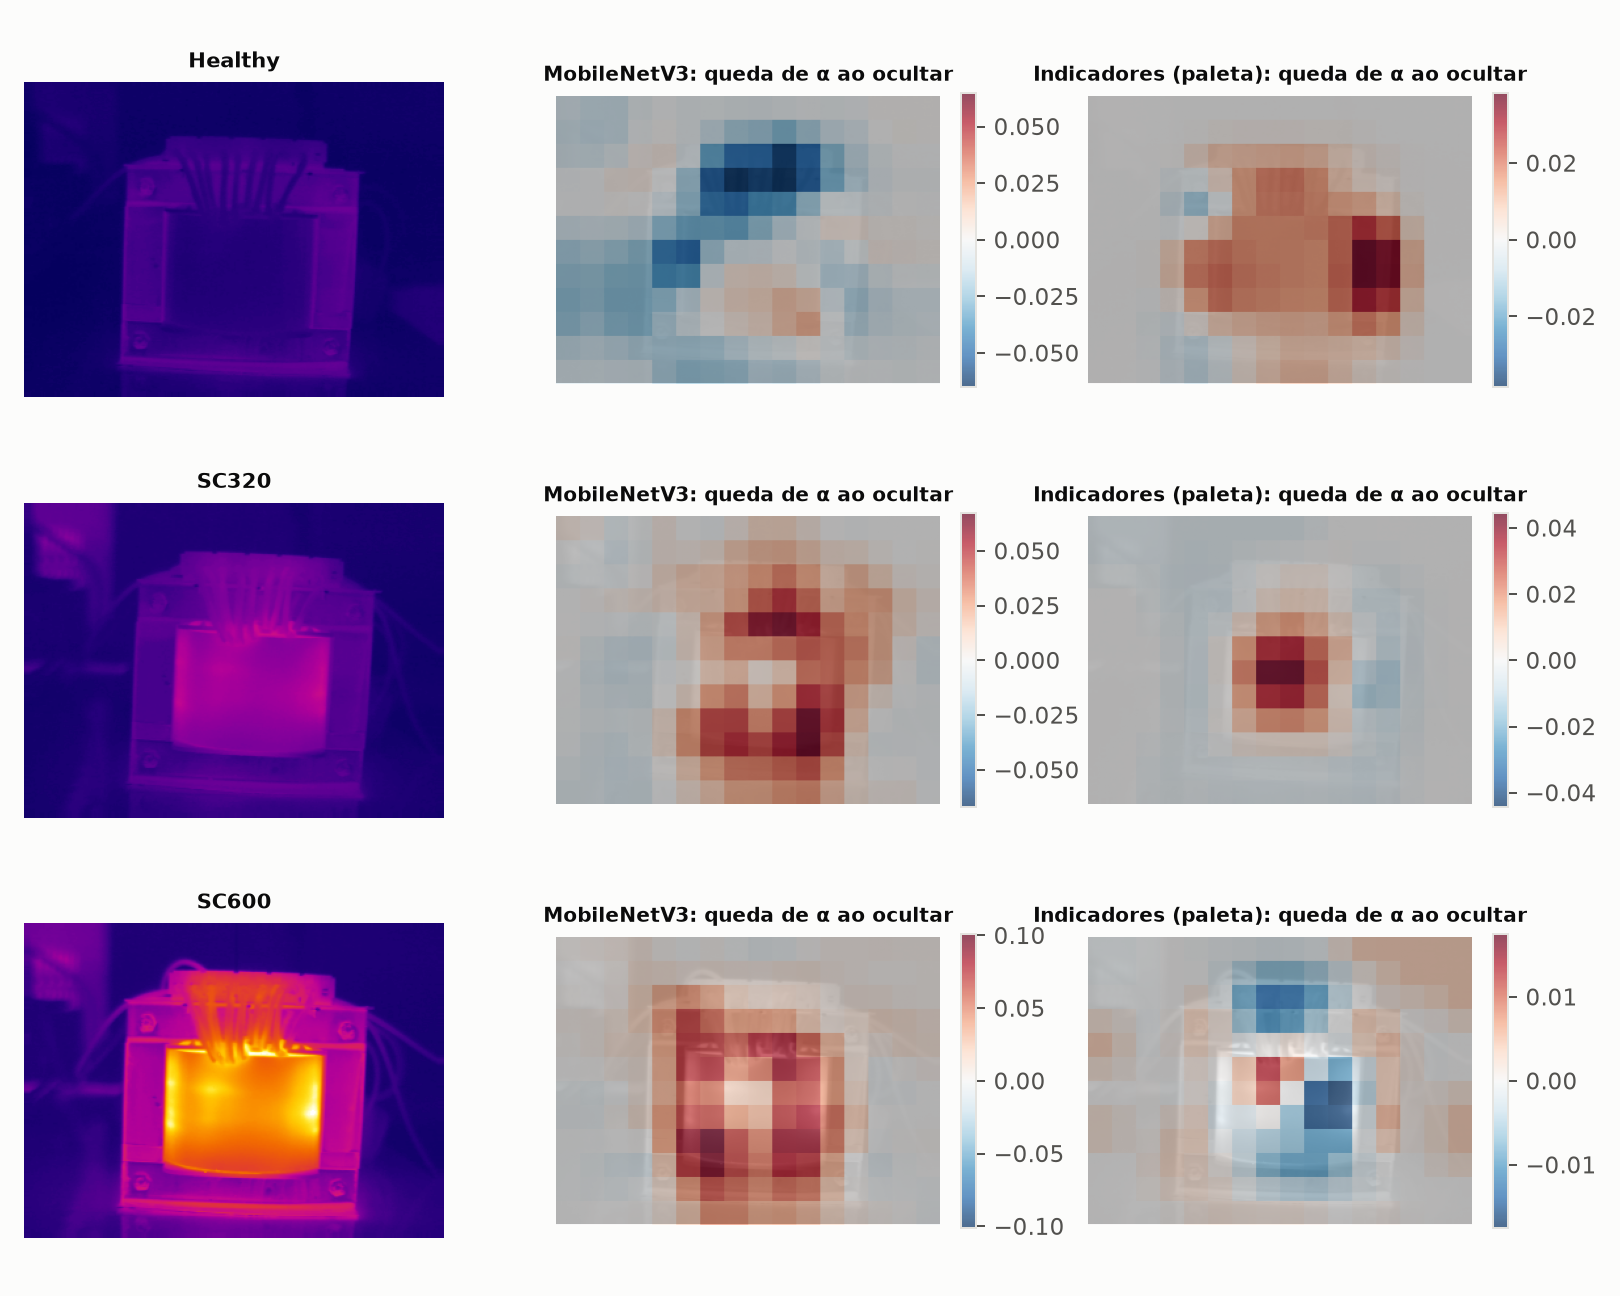
\includegraphics[width=0.75\linewidth]{fig_oclusao.png}
\caption{Queda do $\alpha$ previsto ao ocultar cada região da imagem com a cor do fundo \cite{zeiler2014}, para uma imagem saudável, uma do SC320 e uma do SC600.}
\label{fig:oclusao}
\end{figure}

Na análise de oclusão (Fig.~\ref{fig:oclusao}), de \OclMobMin{} a \OclMobMax{} da queda de $\hat\alpha$ da MobileNetV3 ocorreram ao ocultar a região do transformador, e não o fundo. Para o modelo de indicadores, a fração variou de \OclIndMin{} a \OclIndMax{}; no SC600, parte do efeito veio de fora da região segmentada, o que reforça a cautela com indicadores que dependem da cena.

\subsection{Segundo equipamento: motor de indução}
O mesmo pipeline, sem ajustes, foi aplicado aos 369 termogramas do motor de indução do mesmo dataset \cite{najafi2020motor}, com 11 condições (sem carga, rotor travado, falha do ventilador e oito combinações de curto no estator). A paleta também foi recuperada sem rótulos (\MotorCores{} cores). A classificação por blocos temporais atingiu F1-macro de \MotorFUm{} (linha de base: \MotorFUmTriv{}; controle de posição: \MotorFUmPos). Definindo a severidade do estator como a fração total de espiras em curto (porcentagem por fase vezes número de fases, dividido por três), o erro dentro das sessões foi de \MotorMAE{} ponto percentual (Tabela~\ref{tab:motor}). No teste de severidade não vista, porém, o controle de posição (\MotorSevPos{} p.p.) errou menos que a MobileNetV3 (\MotorSevMob{} p.p.): no motor, a sequência de gravação acompanha a severidade e o enquadramento muda gradualmente, e o teste não discrimina métodos. O pipeline é portanto transferível para classificação e severidade dentro das sessões, mas a generalização a sessões novas no motor não pode ser avaliada com esses dados.

\begin{table}[t]
\centering
\caption{Motor de indução: F1-macro das 11 condições (blocos) e erro da severidade do estator em pontos percentuais}
\label{tab:motor}
\small\begin{tabular}{lrrrr}
\toprule
Features & F1 (11 cond.) & MAE blocos & MAE sev. nova & Pior \\
\midrule
Miniatura 16$\times$12 (linha de base) & 0,942 & 1,47 & 6,0 & 17,5 \\
Posição do objeto (controle) & 0,542 & 4,45 & 3,8 & 8,8 \\
Indicadores de paleta & 0,992 & 1,31 & 5,1 & 10,6 \\
MobileNetV3 & 0,988 & 0,97 & 4,1 & 10,1 \\
MobileNetV3 + indicadores de paleta & 0,997 & 0,85 & 4,4 & 10,7 \\
\bottomrule
\end{tabular}

\end{table}

\subsection{Camada de relatório}
Os \RelAprovados{} relatórios gerados a partir dos registros foram aprovados pelo verificador. Para medir a sensibilidade do verificador, sete tipos de erro foram injetados em cada relatório (Tabela~\ref{tab:verificador}). Os erros numéricos e de conteúdo foram detectados em \VerifMin{} a \VerifMax{} dos casos. A afirmação sobre vida útil, que não contém número, gerou apenas alerta. A limitação conhecida do verificador é conferir a existência de cada número no registro, e não a qual campo ele se refere. \todo{acrescentar os resultados de main.py --llm claude: quantos relatórios reais do LLM foram aprovados e por que os reprovados falharam}

\begin{table}[t]
\centering
\caption{Sensibilidade do verificador a erros injetados}
\label{tab:verificador}
\small\begin{tabular}{lr}
\toprule
Erro injetado (255 relatórios cada) & Detectado \\
\midrule
Temperatura inventada (``87\,\textdegree C'') & 100,0\% \\
Corrente inventada (``3,2\,A'') & 100,0\% \\
Espiras recalculadas & 100,0\% \\
Recomendação trocada & 100,0\% \\
Limitações omitidas & 100,0\% \\
$\alpha$ alterado & 99,2\% \\
``Reduz a vida útil'' (alerta) & 100,0\% \\
\bottomrule
\end{tabular}

\end{table}

\section{Aplicação}
O pipeline foi empacotado em uma ferramenta de linha de comando e em uma interface web local. O usuário envia um termograma e recebe a condição estimada, $\hat\alpha$ com intervalo de 90\% (meia-largura de \AppMeia{} espiras, calibrada para severidade nova), o aviso de domínio, a recomendação e o relatório verificado. O modelo de aplicação usa a MobileNetV3 com aumento de dados, que roda sem acesso à internet após a instalação. Um termograma do motor de indução submetido ao modelo do transformador foi marcado como fora do domínio, e a recomendação foi substituída pelo encaminhamento a um especialista.

\section{Conclusões}
Em termogramas não radiométricos de um transformador de bancada, a combinação de DINOv2 com indicadores calculados sobre o índice de paleta estimou severidades ausentes do treinamento com erro médio de \InterpHib{} espiras de 600, com ganho significativo sobre cada componente isolado. A avaliação dentro das sessões de gravação, usada no estudo preliminar, mostrou-se pouco informativa, pois até uma linha de base trivial atinge o teto. A generalização a novas campanhas de aquisição foi mais difícil (\CampHib{} espiras) e a extrapolação para fora da faixa de severidades treinada não foi possível; nesses casos, o detector de domínio sinalizou a maior parte das imagens. A camada de relatório por LLM, restrita a redigir o diagnóstico estruturado e verificada automaticamente, tornou auditável a etapa mais sujeita a erros de linguagem.

Os resultados são condicionados a um único equipamento de bancada, a curtos provocados, a imagens sem radiometria e a uma única campanha com a condição saudável. Trabalhos futuros devem incluir imagens radiométricas, medições elétricas por ensaio, campanhas independentes para cada condição e validação entre equipamentos.

\bibliographystyle{unsrt}
\bibliography{referencias}

\end{document}
